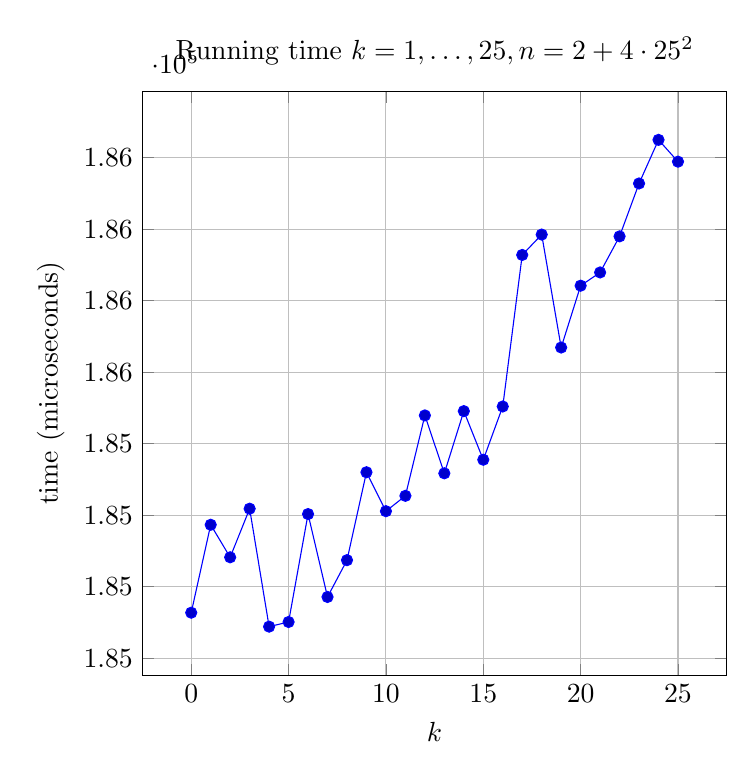
\begin{tikzpicture}
\begin{axis}[
title={Running time $k=1,\dots,25,n=2+4\cdot 25^2$},
height=9cm,
width=9cm,
grid=major,
xlabel = $k$,
ylabel = time (microseconds),
]

\addplot coordinates {
	(0,184927)
	(1,185173)
	(2,185082)
	(3,185218)
	(4,184888)
	(5,184901)
	(6,185203)
	(7,184971)
	(8,185074)
	(9,185320)
	(10,185211)
	(11,185254)
	(12,185479)
	(13,185317)
	(14,185491)
	(15,185355)
	(16,185504)
	(17,185928)
	(18,185985)
	(19,185669)
	(20,185842)
	(21,185879)
	(22,185980)
	(23,186128)
	(24,186250)
	(25,186189)
};
\end{axis}
\end{tikzpicture}
